\scanpage{5}
Voorschoten, March 29 1967\\
Palestrinalaan 11\\

Dear Grothendieck,\\

Enclosed I send you - finally - ,in two different covers, the manuscript on the tame fund. group together with the papers which I borrowed from you.

As to the terminology: I have used scheme in stead of prescheme (without mentioning it because I expect this will be \deleted{\unsure{f}}\inserted{a} general remark in SGA I) but I have not used ``doublet'' because I don't know your final decision on this point.
\margin{\figure{
\begin{tikzpicture}[scale=.8]\node[rotate=31] at (-.65,0) {stroke};\draw (.4,-.25)--(.4,.45);\end{tikzpicture}}}

References: I have made freely references to EGA (also to EGA IV) \uline{but only to SGA 1960/61} (with one notable misleading : a reference to SGA X, Cor 3.3 etc, the purity theorem, is a misleading because the proof is only in SGA 1962). I don't know the `new numbering' of SGA (You mentioned something about it, but I don't remember) so I have used still SGA I, SGA V etc for the 1960/61 séminaire.
\margin{SGA 1}

I must admit that there are still many points which are not satisfactory in the exposition. Below are some comments, motivations and questions:

p.3 Hyp.1\quad Perhaps it would have been nicer to avoid a little longer this assumption. However there is in SGA 1960/61 only a statement about quotients and existence of quotients in case the group is an \uline{ordinary} finite group (it is only in SGA D that the theorems from TDTE III are proved and the proof is long and subtle!) This is the reason for making the assumption Hyp 1 already here.

p.5. line 6 below:\quad the emphasis on $H$ ordinary group : same reason

p.6 (Cor 1.11)\quad \uline{In fact this is a general question} : I have hesitated a little bit \unsure{W|w}ith the word ``covering'' for ``revêtement'' (of course: already used in the title!)
\margin{\figure{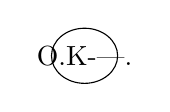
\begin{tikzpicture}[scale=.7]\draw (0,0) ellipse (.6 and .5);\node at (0,0) {O.K\unsure{-|.}};\end{tikzpicture}}}
Originally revêtement was used as translation \deleted{for covering} (in Serre\unsure{.|-}Lang's paper) for covering (in Lang's paper)!\unsure{.} But now there may be confusion with ``covering in some topology'' for instance ``covering in the étale topology'' which is something entirely different. What do you think about this? I don't see what
\margin{O.K.}
% archive sheet number: 4
